\section{Monday for MAT4002}\index{Monday_lecture}
\begin{proposition}
If $b,b'$ are path connected in $X$, then
\[
\pi_1(X,b)\cong \pi_1(X,b')
\]
\end{proposition}
\begin{remark}
Last lecture we have given the isomorphism
\[
\begin{array}{ll}
W_{\#}:&\pi_1(X,b)\to \pi_1(X,b')\\
\text{with}&[\ell]\mapsto[w^{-1}\cdot \ell \cdot w]
\end{array}
\]
where $w$ denotes a path from $b$ to $b'$.
The inverse of $W_{\#}$ is given by:
\[
\begin{array}{ll}
W^{-1}_{\#}:&\pi_1(X,b')\to \pi_1(X,b)\\
\text{with}&[m]\mapsto[w\cdot m \cdot w^{-1}]
\end{array}
\]
\end{remark}
\paragraph{Notation}
For path connected space $X$, we will just write $\pi_1(X)$ instead of $\pi_1(X,x)$.


\begin{proposition}\label{pro:12:4}
Let $(X,x)$ and $(Y,y)$ be spaces with basepoints $x$ and $y$, and $f:X\to Y$ be a continuous map with $f(x)=y$. Then every loop $\ell:I\to X$ based at $x$ gives a loop $f\circ\ell:I\to Y$ based at $y$, i.e., the continous map $f$ induces a homomorphism of groups
\[
\begin{array}{ll}
f_*:&\pi_1(\pi,x)\to\pi_1(Y,y)\\
&[\ell]\mapsto[f\circ\ell]:=f_*([\ell])
\end{array}
\]
Moreover,
\begin{enumerate}
\item
$(\text{id}_{X\to X})_*=\text{id}_{\pi_1(X,x)\to \pi_1(X,x)}$
\item
$(g\circ f)_* = g_*\circ f_*$
\item
If $f\simeq f'$ relative to $x\in X$, then $f_*=(f')_*$
\end{enumerate}
\end{proposition}
\begin{proof}
\begin{itemize}
\item
Well-definedness: 
Suppose that $\ell\simeq\ell'$, then $f\circ \ell\simeq f\circ\ell'$ by propositon~(\ref{pro:9:4}).
Therefore, $[f\circ\ell]=[f\circ\ell']$.
\item
Homomorphism:
It's clear that
\[
f\circ(\ell\circ \ell') = (f\circ\ell)\circ(f\circ \ell')
\]
Therefore, $f_*[\ell\ell']=(f_*[\ell])*(f_*[\ell'])$
\end{itemize}
The other three statements are obvious.

\end{proof}


\begin{proposition}\label{pro:12:5}
Let $X,Y$ be path-connected such that $X\simeq Y$ (i.e., there exists $f:X\to Y$ and $g:Y\to X$ such that $g\circ f\simeq\text{id}_X,f\circ g\simeq\text{id}_Y$).
Then $\pi_1(X)\cong\pi_1(Y)$.

In particular, if $X,Y$ are path-connected with $X\cong Y$, then $\pi_1(X)\cong\pi_1(Y)$
\end{proposition}
\begin{proof}
Consider the mapping
\[
\pi_1(X,x_0)\xrightarrow{f_*}\pi_1(Y,y_0)\xrightarrow{g_*}
\pi_1(X,x_1)
\]
It suffices to show that $f_*$ and $g_*$ are bijective. (The homomorphism follows from proposition~(\ref{pro:12:4}))
\begin{itemize}
\item
Wrong proof: $g\circ f\simeq\text{id}_X$ implies $(g\circ f)_*=(\text{id}_X)_*$ implies $g_*\circ f_*=\text{id}_{\pi_1(X,x_0)}$.

Reason: note that $(g\circ f)\simeq\text{id}_X$ is \emph{not} relative to $x_0$.
\end{itemize}

Consider the homotopy $H:g\circ f\simeq\text{id}_X$, where $H(x_0,s)$ is not necessarily a constant for $s\in I$.
It follows that $H(x_0,0)=x_1$ and $H(x_0,1)=x_0$, i.e., $w(s):=H(x_0,s)$ defines a path from $x_1$ to $x_0$.

For any loop $\ell:I\to X$ based at $x_0$, consider the homotopy 
\[
\begin{array}{ll}
K=H\circ(\ell\times\text{id}_I):&I\times I\to X\\
\text{where}&K(t,s) = H((\ell(t),s))\\
&K(t,0)=H(\ell(t),0) = g\circ f(\ell(t))\\
&K(t,1)=H(\ell(t),1) = \ell(t)\\
&K(0,s)=w(s)=K(1,s)
\end{array}
\]
The graphic plot of $K$ is given in the figure below:
\begin{figure}[H]
\centering
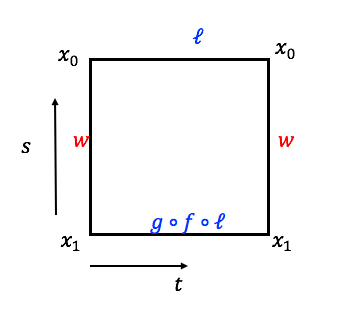
\includegraphics[width=0.5\textwidth]{week12/f_12_5}
\end{figure}
The homotopy between $\ell$ and $g\circ f\circ\ell$ motivates us to construct a homotopy between $\ell$ and $w^{-1}\circ g\circ f\circ \ell\circ w$ relative to $\{0,1\}$:
\begin{figure}[H]
\centering
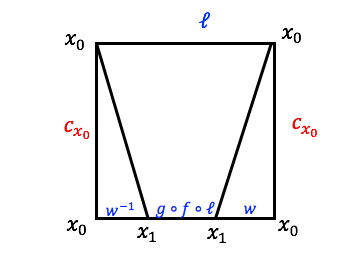
\includegraphics[width=0.5\textwidth]{week12/f_12_6}
\end{figure}
Therefore,
\[
[\ell]=[w^{-1}gf\ell w] = W_{\#}([gf\ell])=(W_{\#}\circ g_*\circ f_*)[\ell]
\]
which follows that $W_{\#}\circ g_*\circ f_*=\text{id}_{\pi_1(X,x_0)}$. Therfore, $f_*$ is injective, $g_*$ is surjective.

The similar argument gives 
\[
W_{\#}\circ f_*\circ g_* = \text{id}_{\pi_1(Y,y_0)}
\]
Therefore, $f_*$ is surjective, $g_*$ is injective. The bijectivity is shown.

\end{proof}

\begin{definition}[Simply-Connected]
A space $X$ is \emph{simply-connected} if $X$ is path connected, and $X$ has trivial fundamental group, i.e., $\pi_1(X)=\{e\}$ for some point $e\in X$.
\end{definition}

\begin{example}
If $X$ is contractible, then $X$ is path-connected.
By proposition~(\ref{pro:12:5}), since $X\simeq\{e\}$, we imply
\[
\pi_1(X)\cong\pi_1(\{e\})=\{e\}.
\]
Therefore, all contractible spaces (e.g., $\mathbb{R}^n$) are simply-connected.

However, not all simply-connected spaces are contractible, e.g., $\pi_1(S^2)\cong\{e\}$, but $S^2$ is not homotopy equivalent to a point.
\end{example}


\subsection{Some basic results on $\pi_1(X,b)$}



We will study $\pi_1(X,b)$ for some simplicial complexes.
\begin{definition}[Edge Loop]
Let $K=(V,\Sigma)$ be a simplicial complex.
\begin{enumerate}
\item
An edge path $(v_0,\dots,v_n)$ is such that
\begin{enumerate}
\item
$a_i\in V(K)$
\item
For each $i$, $\{a_{i-1},a_i\}$ spans a simplex of $K$
\end{enumerate}
\item
An edge loop is an edge path with $a_n=a_0$.
\item
Let $\alpha = (v_0,\dots,v_n),\beta = (w_0,\dots,w_m)$ be two edge paths with $v_n=w_0$, then we define 
\[
\alpha\circ\beta =(v_0,\dots,v_n,w_1,\dots,w_m)
\]
\end{enumerate}
\end{definition}




\begin{definition}[Elementary Contraction/Expansion]
Let $\alpha,\beta$ be two edge paths.
\begin{enumerate}
\item
An elementary contraction of $\alpha$ is a new edge path obtained by performing one of the followings on $\alpha$:
\begin{itemize}
\item
Replacing $\cdots a_{i-1}a_i\cdots$ by $\cdots a_{i-1}\cdots$ provided that $a_{i-1}=a_i$
\item
Replacing $\cdots a_{i-1}a_ia_{i+1}\cdots$ by $\cdots a_{i-1}\cdots$ provided that $a_{i-1}=a_{i+1}$
\item
Replacing $\cdots a_{i-1}a_ia_{i+1}\cdots$ by $\cdots a_{i-1}a_{i+1}\cdots$ provided that $\{a_{i-1},a_i,a_{i+1}\}$ spans a $2$-simplex of $K$.
\end{itemize}
\item
An elementary expansion is the reverse of the elementary contraction.
\item
Two edge paths $\alpha,\beta$ are equivalent if $\alpha$ and $\beta$ differs by a finite sequence of elementary contractions or expansions.
\end{enumerate}
\end{definition}















